\chapter{Busca completa}

\key{Busca completa}
é um método geral que pode ser usado
para resolver quase qualquer problema algorítmico.
A ideia é gerar todas as soluções possíveis
para o problema usando força bruta,
e então selecionar a melhor solução ou contar o
número de soluções, dependendo do problema.

A busca completa é uma boa técnica
se houver tempo suficiente para verificar todas as soluções,
porque a busca é geralmente fácil de implementar
e sempre fornece a resposta correta.
Se a busca completa for muito lenta,
outras técnicas, como algoritmos gulosos ou
programação dinâmica, podem ser necessárias.

\section{Gerando subconjuntos}

\index{subset}

Consideramos primeiro o problema de gerar
todos os subconjuntos de um conjunto de $n$ elementos.
Por exemplo, os subconjuntos de $\{0,1,2\}$ são
$\emptyset$, $\{0\}$, $\{1\}$, $\{2\}$, $\{0,1\}$,
$\{0,2\}$, $\{1,2\}$ e $\{0,1,2\}$.
Existem dois métodos comuns para gerar subconjuntos:
podemos realizar uma busca recursiva
ou explorar a representação de bits de inteiros.

\subsubsection{Método 1}

Uma maneira elegante de percorrer todos os subconjuntos
de um conjunto é usar recursão.
A seguinte função \texttt{search}
gera os subconjuntos do conjunto
$\{0,1,\ldots,n-1\}$.
A função mantém um vetor \texttt{subset}
que conterá os elementos de cada subconjunto.
A busca começa quando a função é chamada
com o parâmetro 0.

\begin{lstlisting}
void search(int k) {
    if (k == n) {
        // processa subconjunto
    } else {
        search(k+1);
        subset.push_back(k);
        search(k+1);
        subset.pop_back();
    }
}
\end{lstlisting}

Quando a função \texttt{search}
é chamada com o parâmetro $k$,
ela decide se inclui o
elemento $k$ no subconjunto ou não,
e em ambos os casos,
então chama a si mesma com o parâmetro $k+1$.
No entanto, se $k=n$, a função percebe que
todos os elementos foram processados
e um subconjunto foi gerado.

A seguinte árvore ilustra as chamadas de função quando $n=3$.
Podemos sempre escolher o ramo esquerdo
($k$ não está incluído no subconjunto) ou o ramo direito
($k$ está incluído no subconjunto).

\begin{center}
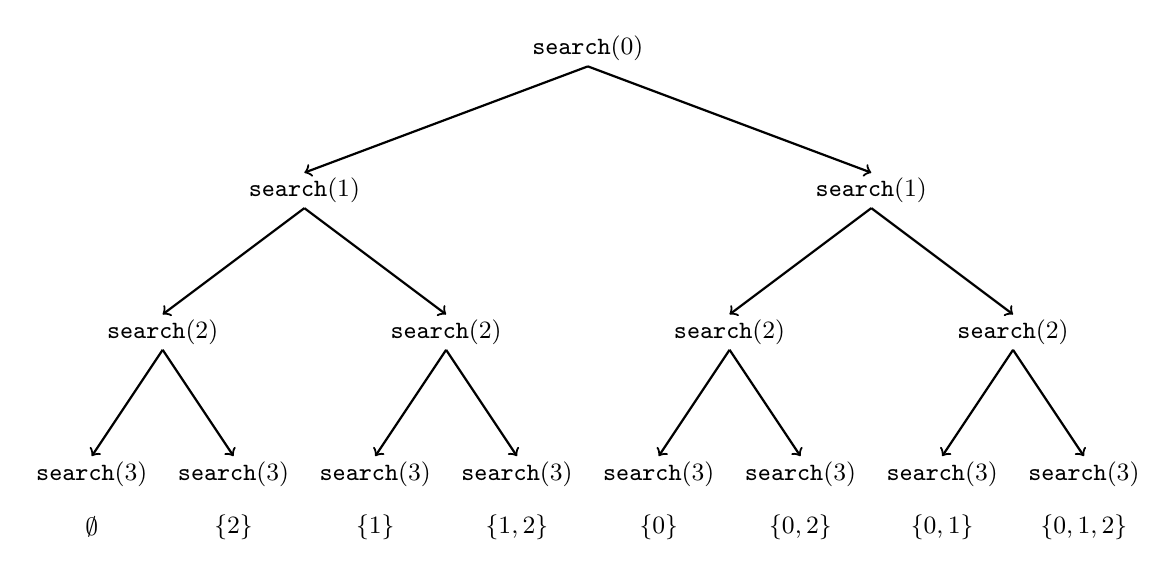
\begin{tikzpicture}[scale=.45]
  \begin{scope}
    \small
    \node at (0,0) {$\texttt{search}(0)$};

    \node at (-8,-4) {$\texttt{search}(1)$};
    \node at (8,-4) {$\texttt{search}(1)$};

    \path[draw,thick,->] (0,0-0.5) -- (-8,-4+0.5);
    \path[draw,thick,->] (0,0-0.5) -- (8,-4+0.5);

    \node at (-12,-8) {$\texttt{search}(2)$};
    \node at (-4,-8) {$\texttt{search}(2)$};
    \node at (4,-8) {$\texttt{search}(2)$};
    \node at (12,-8) {$\texttt{search}(2)$};

    \path[draw,thick,->] (-8,-4-0.5) -- (-12,-8+0.5);
    \path[draw,thick,->] (-8,-4-0.5) -- (-4,-8+0.5);
    \path[draw,thick,->] (8,-4-0.5) -- (4,-8+0.5);
    \path[draw,thick,->] (8,-4-0.5) -- (12,-8+0.5);

    \node at (-14,-12) {$\texttt{search}(3)$};
    \node at (-10,-12) {$\texttt{search}(3)$};
    \node at (-6,-12) {$\texttt{search}(3)$};
    \node at (-2,-12) {$\texttt{search}(3)$};
    \node at (2,-12) {$\texttt{search}(3)$};
    \node at (6,-12) {$\texttt{search}(3)$};
    \node at (10,-12) {$\texttt{search}(3)$};
    \node at (14,-12) {$\texttt{search}(3)$};

    \node at (-14,-13.5) {$\emptyset$};
    \node at (-10,-13.5) {$\{2\}$};
    \node at (-6,-13.5) {$\{1\}$};
    \node at (-2,-13.5) {$\{1,2\}$};
    \node at (2,-13.5) {$\{0\}$};
    \node at (6,-13.5) {$\{0,2\}$};
    \node at (10,-13.5) {$\{0,1\}$};
    \node at (14,-13.5) {$\{0,1,2\}$};


    \path[draw,thick,->] (-12,-8-0.5) -- (-14,-12+0.5);
    \path[draw,thick,->] (-12,-8-0.5) -- (-10,-12+0.5);
    \path[draw,thick,->] (-4,-8-0.5) -- (-6,-12+0.5);
    \path[draw,thick,->] (-4,-8-0.5) -- (-2,-12+0.5);
    \path[draw,thick,->] (4,-8-0.5) -- (2,-12+0.5);
    \path[draw,thick,->] (4,-8-0.5) -- (6,-12+0.5);
    \path[draw,thick,->] (12,-8-0.5) -- (10,-12+0.5);
    \path[draw,thick,->] (12,-8-0.5) -- (14,-12+0.5);
\end{scope}
\end{tikzpicture}
\end{center}

\subsubsection{Método 2}

Outra maneira de gerar subconjuntos é baseada na
representação de bits de inteiros.
Cada subconjunto de um conjunto de $n$ elementos
pode ser representado como uma sequência de $n$ bits,
que corresponde a um inteiro entre $0 \ldots 2^n-1$.
Os uns na sequência de bits indicam
quais elementos estão incluídos no subconjunto.

A convenção usual é que
o último bit corresponde ao elemento 0,
o penúltimo bit corresponde ao elemento 1,
e assim por diante.
Por exemplo, a representação de bits de 25
é 11001, que corresponde ao subconjunto $\{0,3,4\}$.

O seguinte código percorre os subconjuntos
de um conjunto de $n$ elementos:

\begin{lstlisting}
for (int b = 0; b < (1<<n); b++) {
    // processa subconjunto
}
\end{lstlisting}

O seguinte código mostra como podemos encontrar
os elementos de um subconjunto que corresponde a uma sequência de bits.
Ao processar cada subconjunto,
o código constrói um vetor que contém os
elementos no subconjunto.

\begin{lstlisting}
for (int b = 0; b < (1<<n); b++) {
    vector<int> subset;
    for (int i = 0; i < n; i++) {
        if (b&(1<<i)) subset.push_back(i);
    }
}
\end{lstlisting}

\section{Gerando permutações}

\index{permutation}

A seguir, consideramos o problema de gerar
todas as permutações de um conjunto de $n$ elementos.
Por exemplo, as permutações de $\{0,1,2\}$ são
$(0,1,2)$, $(0,2,1)$, $(1,0,2)$, $(1,2,0)$,
$(2,0,1)$ e $(2,1,0)$.
Novamente, existem duas abordagens:
podemos usar recursão ou percorrer as
permutações iterativamente.

\subsubsection{Método 1}

Assim como os subconjuntos, as permutações podem ser geradas
usando recursão.
A seguinte função \texttt{search} percorre
as permutações do conjunto $\{0,1,\ldots,n-1\}$.
A função constrói um vetor \texttt{permutation}
que contém a permutação,
e a busca começa quando a função é
chamada sem parâmetros.

\begin{lstlisting}
void search() {
    if (permutation.size() == n) {
        // processa permutacao
    } else {
        for (int i = 0; i < n; i++) {
            if (chosen[i]) continue;
            chosen[i] = true;
            permutation.push_back(i);
            search();
            chosen[i] = false;
            permutation.pop_back();
        }
    }
}
\end{lstlisting}

Cada chamada de função adiciona um novo elemento a
\texttt{permutation}.
O array \texttt{chosen} indica quais
elementos já estão incluídos na permutação.
Se o tamanho de \texttt{permutation} for igual ao tamanho do conjunto,
uma permutação foi gerada.

\subsubsection{Método 2}

\index{next\_permutation@\texttt{next\_permutation}}

Outro método para gerar permutações
é começar com a permutação
$\{0,1,\ldots,n-1\}$ e repetidamente
usar uma função que constrói a próxima permutação
em ordem crescente.
A biblioteca padrão C++ contém a função
\texttt{next\_permutation} que pode ser usada para isso:

\begin{lstlisting}
vector<int> permutation;
for (int i = 0; i < n; i++) {
    permutation.push_back(i);
}
do {
    // processa permutacao
} while (next_permutation(permutation.begin(),permutation.end()));
\end{lstlisting}

\section{Backtracking}

\index{backtracking}

Um algoritmo de \key{backtracking}
começa com uma solução vazia
e estende a solução passo a passo.
A busca percorre recursivamente
todas as maneiras diferentes de como
uma solução pode ser construída.

\index{queen problem}

Como exemplo, considere o problema de
calcular o número
de maneiras pelas quais $n$ rainhas podem ser colocadas em
um tabuleiro de xadrez $n \times n$ para que
nenhuma rainha ataque a outra.
Por exemplo, quando $n=4$,
existem duas soluções possíveis:

\begin{center}
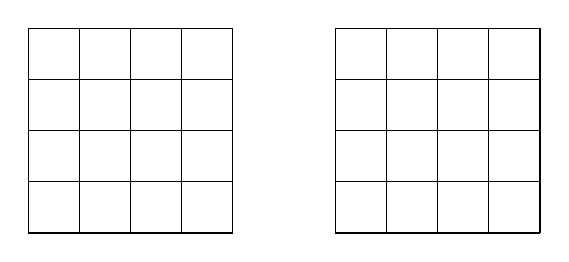
\begin{tikzpicture}[scale=.65]
  \begin{scope}
    \draw (0, 0) grid (4, 4);
    \node at (1.5,3.5) {\symqueen};
    \node at (3.5,2.5) {\symqueen};
    \node at (0.5,1.5) {\symqueen};
    \node at (2.5,0.5) {\symqueen};

    \draw (6, 0) grid (10, 4);
    \node at (6+2.5,3.5) {\symqueen};
    \node at (6+0.5,2.5) {\symqueen};
    \node at (6+3.5,1.5) {\symqueen};
    \node at (6+1.5,0.5) {\symqueen};

  \end{scope}
\end{tikzpicture}
\end{center}

O problema pode ser resolvido usando backtracking
colocando rainhas no tabuleiro linha por linha.
Mais precisamente, exatamente uma rainha será
colocada em cada linha para que nenhuma rainha ataque
qualquer uma das rainhas colocadas anteriormente.
Uma solução foi encontrada quando todas
as $n$ rainhas foram colocadas no tabuleiro.

Por exemplo, quando $n=4$,
alguma solução parcial gerada pelo
algoritmo de backtracking é a seguinte:

\begin{center}
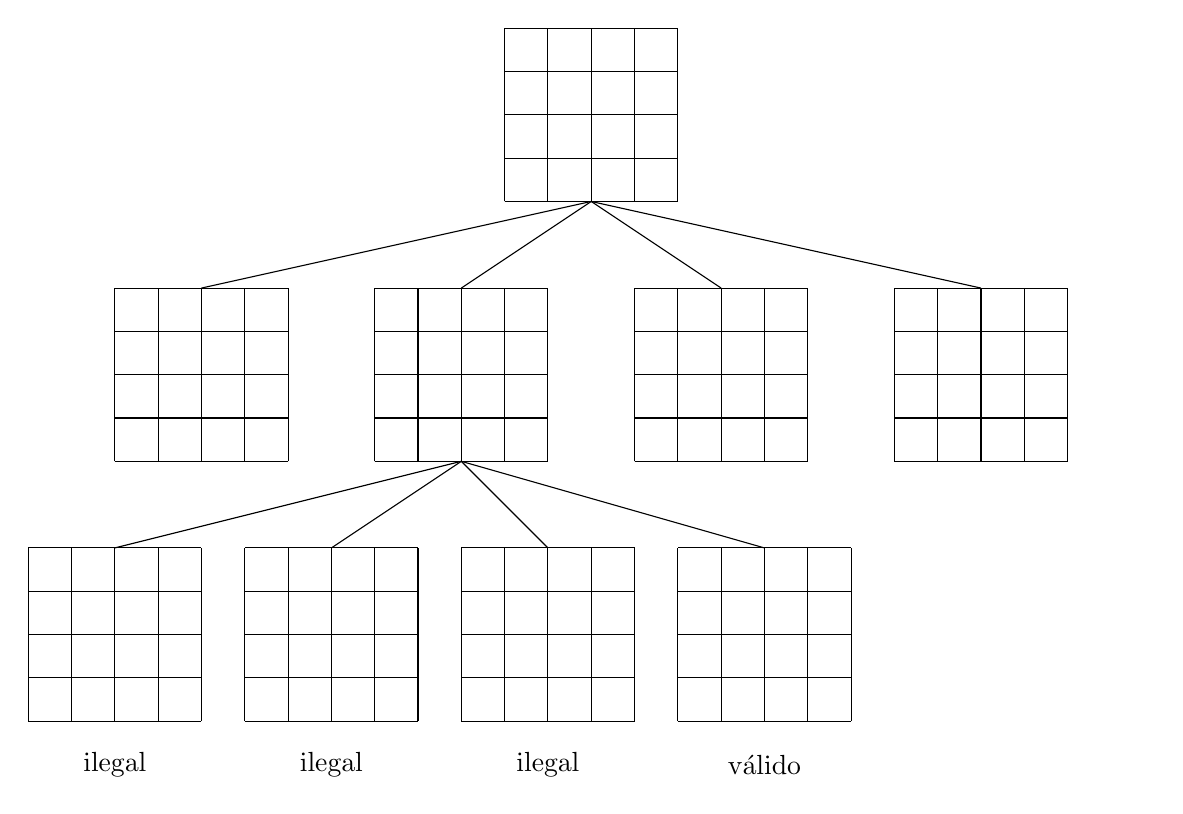
\begin{tikzpicture}[scale=.55]
  \begin{scope}
    \draw (0, 0) grid (4, 4);

    \draw (-9, -6) grid (-5, -2);
    \draw (-3, -6) grid (1, -2);
    \draw (3, -6) grid (7, -2);
    \draw (9, -6) grid (13, -2);

    \node at (-9+0.5,-3+0.5) {\symqueen};
    \node at (-3+1+0.5,-3+0.5) {\symqueen};
    \node at (3+2+0.5,-3+0.5) {\symqueen};
    \node at (9+3+0.5,-3+0.5) {\symqueen};

    \draw (2,0) -- (-7,-2);
    \draw (2,0) -- (-1,-2);
    \draw (2,0) -- (5,-2);
    \draw (2,0) -- (11,-2);

    \draw (-11, -12) grid (-7, -8);
    \draw (-6, -12) grid (-2, -8);
    \draw (-1, -12) grid (3, -8);
    \draw (4, -12) grid (8, -8);
    \draw[white] (11, -12) grid (15, -8);
    \node at (-11+1+0.5,-9+0.5) {\symqueen};
    \node at (-6+1+0.5,-9+0.5) {\symqueen};
    \node at (-1+1+0.5,-9+0.5) {\symqueen};
    \node at (4+1+0.5,-9+0.5) {\symqueen};
    \node at (-11+0+0.5,-10+0.5) {\symqueen};
    \node at (-6+1+0.5,-10+0.5) {\symqueen};
    \node at (-1+2+0.5,-10+0.5) {\symqueen};
    \node at (4+3+0.5,-10+0.5) {\symqueen};

    \draw (-1,-6) -- (-9,-8);
    \draw (-1,-6) -- (-4,-8);
    \draw (-1,-6) -- (1,-8);
    \draw (-1,-6) -- (6,-8);

    \node at (-9,-13) {ilegal};
    \node at (-4,-13) {ilegal};
    \node at (1,-13) {ilegal};
    \node at (6,-13) {válido};

  \end{scope}
\end{tikzpicture}
\end{center}

No nível inferior, as três primeiras configurações
são ilegais, porque as rainhas se atacam.
No entanto, a quarta configuração é válida
e pode ser estendida para uma solução completa por
colocando mais duas rainhas no tabuleiro.
Existe apenas uma maneira de colocar as duas rainhas restantes.

\begin{samepage}
O algoritmo pode ser implementado da seguinte forma:
\begin{lstlisting}
void search(int y) {
    if (y == n) {
        count++;
        return;
    }
    for (int x = 0; x < n; x++) {
        if (column[x] || diag1[x+y] || diag2[x-y+n-1]) continue;
        column[x] = diag1[x+y] = diag2[x-y+n-1] = 1;
        search(y+1);
        column[x] = diag1[x+y] = diag2[x-y+n-1] = 0;
    }
}
\end{lstlisting}
\end{samepage}
A busca começa chamando \texttt{search(0)}.
O tamanho do tabuleiro é $n \times n$,
e o código calcula o número de soluções
para \texttt{count}.

O código assume que as linhas e colunas
do tabuleiro são numeradas de 0 a $n-1$.
Quando a função \texttt{search} é
chamada com o parâmetro $y$,
ela coloca uma rainha na linha $y$
e então chama a si mesma com o parâmetro $y+1$.
Então, se $y=n$, uma solução foi encontrada
e a variável \texttt{count} é incrementada em um.

O array \texttt{column} mantém o controle das colunas
que contêm uma rainha,
e os arrays \texttt{diag1} e \texttt{diag2}
mantêm o controle das diagonais.
Não é permitido adicionar outra rainha a uma
coluna ou diagonal que já contém uma rainha.
Por exemplo, as colunas e diagonais do
tabuleiro $4 \times 4$ são numeradas da seguinte forma:

\begin{center}
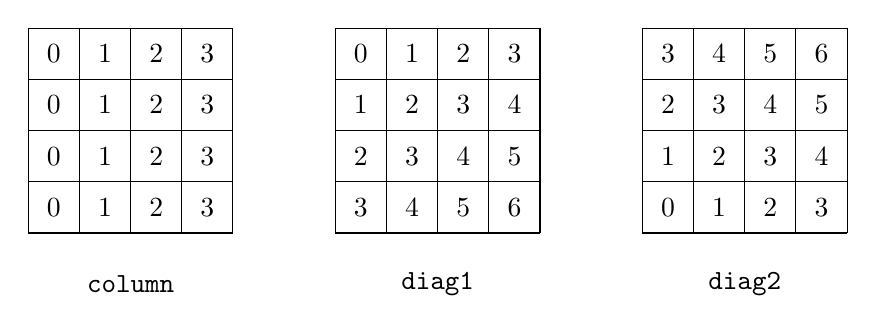
\begin{tikzpicture}[scale=.65]
  \begin{scope}
    \draw (0-6, 0) grid (4-6, 4);
    \node at (-6+0.5,3.5) {$0$};
    \node at (-6+1.5,3.5) {$1$};
    \node at (-6+2.5,3.5) {$2$};
    \node at (-6+3.5,3.5) {$3$};
    \node at (-6+0.5,2.5) {$0$};
    \node at (-6+1.5,2.5) {$1$};
    \node at (-6+2.5,2.5) {$2$};
    \node at (-6+3.5,2.5) {$3$};
    \node at (-6+0.5,1.5) {$0$};
    \node at (-6+1.5,1.5) {$1$};
    \node at (-6+2.5,1.5) {$2$};
    \node at (-6+3.5,1.5) {$3$};
    \node at (-6+0.5,0.5) {$0$};
    \node at (-6+1.5,0.5) {$1$};
    \node at (-6+2.5,0.5) {$2$};
    \node at (-6+3.5,0.5) {$3$};

    \draw (0, 0) grid (4, 4);
    \node at (0.5,3.5) {$0$};
    \node at (1.5,3.5) {$1$};
    \node at (2.5,3.5) {$2$};
    \node at (3.5,3.5) {$3$};
    \node at (0.5,2.5) {$1$};
    \node at (1.5,2.5) {$2$};
    \node at (2.5,2.5) {$3$};
    \node at (3.5,2.5) {$4$};
    \node at (0.5,1.5) {$2$};
    \node at (1.5,1.5) {$3$};
    \node at (2.5,1.5) {$4$};
    \node at (3.5,1.5) {$5$};
    \node at (0.5,0.5) {$3$};
    \node at (1.5,0.5) {$4$};
    \node at (2.5,0.5) {$5$};
    \node at (3.5,0.5) {$6$};

    \draw (6, 0) grid (10, 4);
    \node at (6.5,3.5) {$3$};
    \node at (7.5,3.5) {$4$};
    \node at (8.5,3.5) {$5$};
    \node at (9.5,3.5) {$6$};
    \node at (6.5,2.5) {$2$};
    \node at (7.5,2.5) {$3$};
    \node at (8.5,2.5) {$4$};
    \node at (9.5,2.5) {$5$};
    \node at (6.5,1.5) {$1$};
    \node at (7.5,1.5) {$2$};
    \node at (8.5,1.5) {$3$};
    \node at (9.5,1.5) {$4$};
    \node at (6.5,0.5) {$0$};
    \node at (7.5,0.5) {$1$};
    \node at (8.5,0.5) {$2$};
    \node at (9.5,0.5) {$3$};

    \node at (-4,-1) {\texttt{column}};
    \node at (2,-1) {\texttt{diag1}};
    \node at (8,-1) {\texttt{diag2}};

  \end{scope}
\end{tikzpicture}
\end{center}

Seja $q(n)$ o número de maneiras
de colocar $n$ rainhas em um tabuleiro de xadrez $n \times n$.
O algoritmo de backtracking acima nos diz que, por exemplo, $q(8)=92$.
Quando $n$ aumenta, a busca rapidamente se torna lenta,
porque o número de soluções aumenta
exponencialmente.
Por exemplo, calcular $q(16)=14772512$
usando o algoritmo acima já leva cerca de um minuto
em um computador moderno\footnote{Não há maneira conhecida de calcular com eficiência
valores maiores de $q(n)$. O recorde atual é
$q(27)=234907967154122528$, calculado em 2016 \cite{q27}.}.

\section{Podando a busca}

Muitas vezes podemos otimizar o backtracking
podando a árvore de busca.
A ideia é adicionar ''inteligência'' ao algoritmo
para que ele perceba o mais rápido possível
se uma solução parcial não pode ser estendida
para uma solução completa.
Essas otimizações podem ter um tremendo
efeito na eficiência da busca.

Vamos considerar o problema
de calcular o número de caminhos
em uma grade $n \times n$ do canto superior esquerdo
para o canto inferior direito, de forma que o
caminho visite cada quadrado exatamente uma vez.
Por exemplo, em uma grade $7 \times 7$,
existem 111712 tais caminhos.
Um dos caminhos é o seguinte:

\begin{center}
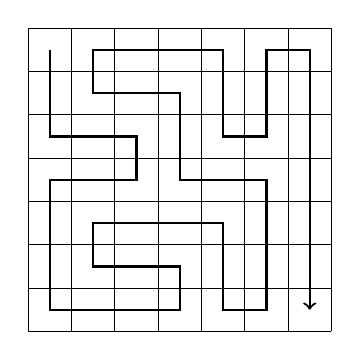
\begin{tikzpicture}[scale=.55]
  \begin{scope}
    \draw (0, 0) grid (7, 7);
    \draw[thick,->] (0.5,6.5) -- (0.5,4.5) -- (2.5,4.5) --
          (2.5,3.5) -- (0.5,3.5) -- (0.5,0.5) --
          (3.5,0.5) -- (3.5,1.5) -- (1.5,1.5) --
          (1.5,2.5) -- (4.5,2.5) -- (4.5,0.5) --
          (5.5,0.5) -- (5.5,3.5) -- (3.5,3.5) --
          (3.5,5.5) -- (1.5,5.5) -- (1.5,6.5) --
          (4.5,6.5) -- (4.5,4.5) -- (5.5,4.5) --
          (5.5,6.5) -- (6.5,6.5) -- (6.5,0.5);
  \end{scope}
\end{tikzpicture}
\end{center}

Vamos nos concentrar no caso $7 \times 7$,
porque seu nível de dificuldade é apropriado às nossas necessidades.
Começamos com um algoritmo de backtracking direto,
e então o otimizamos passo a passo usando observações
de como a busca pode ser podada.
Após cada otimização, medimos o tempo de execução
do algoritmo e o número de chamadas recursivas,
para que possamos ver claramente o efeito de cada
otimização na eficiência da busca.

\subsubsection{Algoritmo básico}

A primeira versão do algoritmo não contém
nenhuma otimização. Nós simplesmente usamos backtracking para gerar
todos os caminhos possíveis do canto superior esquerdo para
o canto inferior direito e contamos o número de tais caminhos.

\begin{itemize}
\item
tempo de execução: 483 segundos
\item
número de chamadas recursivas: 76 bilhões
\end{itemize}

\subsubsection{Otimização 1}

Em qualquer solução, primeiro nos movemos um passo
para baixo ou para a direita.
Há sempre dois caminhos que
são simétricos
sobre a diagonal da grade
após o primeiro passo.
Por exemplo, os seguintes caminhos são simétricos:

\begin{center}
\begin{tabular}{ccc}
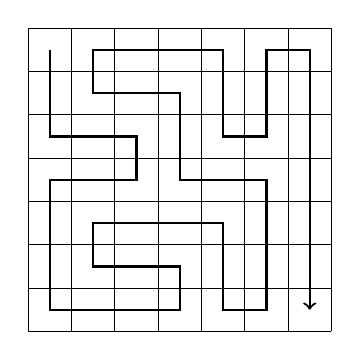
\begin{tikzpicture}[scale=.55]
  \begin{scope}
    \draw (0, 0) grid (7, 7);
    \draw[thick,->] (0.5,6.5) -- (0.5,4.5) -- (2.5,4.5) --
          (2.5,3.5) -- (0.5,3.5) -- (0.5,0.5) --
          (3.5,0.5) -- (3.5,1.5) -- (1.5,1.5) --
          (1.5,2.5) -- (4.5,2.5) -- (4.5,0.5) --
          (5.5,0.5) -- (5.5,3.5) -- (3.5,3.5) --
          (3.5,5.5) -- (1.5,5.5) -- (1.5,6.5) --
          (4.5,6.5) -- (4.5,4.5) -- (5.5,4.5) --
          (5.5,6.5) -- (6.5,6.5) -- (6.5,0.5);
  \end{scope}
\end{tikzpicture}
& \hspace{20px}
& 
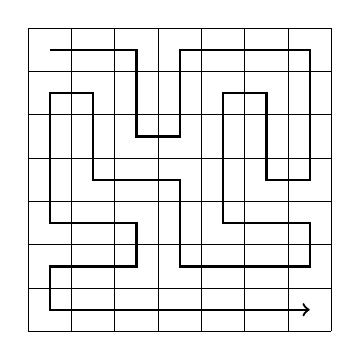
\begin{tikzpicture}[scale=.55]
  \begin{scope}[yscale=1,xscale=-1,rotate=-90]
    \draw (0, 0) grid (7, 7);
    \draw[thick,->] (0.5,6.5) -- (0.5,4.5) -- (2.5,4.5) --
          (2.5,3.5) -- (0.5,3.5) -- (0.5,0.5) --
          (3.5,0.5) -- (3.5,1.5) -- (1.5,1.5) --
          (1.5,2.5) -- (4.5,2.5) -- (4.5,0.5) --
          (5.5,0.5) -- (5.5,3.5) -- (3.5,3.5) --
          (3.5,5.5) -- (1.5,5.5) -- (1.5,6.5) --
          (4.5,6.5) -- (4.5,4.5) -- (5.5,4.5) --
          (5.5,6.5) -- (6.5,6.5) -- (6.5,0.5);
  \end{scope}
\end{tikzpicture}
\end{tabular}
\end{center}

Portanto, podemos decidir que sempre
nos movemos um passo para baixo (ou para a direita),
e finalmente multiplicamos o número de soluções por dois.

\begin{itemize}
\item
tempo de execução: 244 segundos
\item
número de chamadas recursivas: 38 bilhões
\end{itemize}

\subsubsection{Otimização 2}

Se o caminho atingir o quadrado inferior direito
antes de visitar todos os outros quadrados da grade,
é claro que
não será possível completar a solução.
Um exemplo disso é o seguinte caminho:

\begin{center}
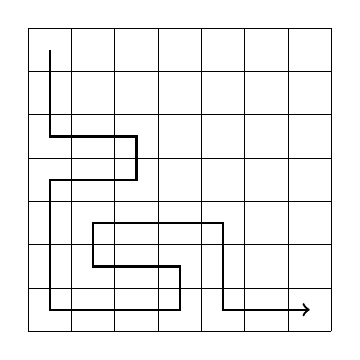
\begin{tikzpicture}[scale=.55]
  \begin{scope}
    \draw (0, 0) grid (7, 7);
    \draw[thick,->] (0.5,6.5) -- (0.5,4.5) -- (2.5,4.5) --
          (2.5,3.5) -- (0.5,3.5) -- (0.5,0.5) --
          (3.5,0.5) -- (3.5,1.5) -- (1.5,1.5) --
          (1.5,2.5) -- (4.5,2.5) -- (4.5,0.5) --
          (6.5,0.5);
  \end{scope}
\end{tikzpicture}
\end{center}
Usando essa observação, podemos encerrar a busca
imediatamente se atingirmos o quadrado inferior direito muito cedo.
\begin{itemize}
\item
tempo de execução: 119 segundos
\item
número de chamadas recursivas: 20 bilhões
\end{itemize}

\subsubsection{Otimização 3}

Se o caminho tocar uma parede
e puder virar à esquerda ou à direita,
a grade se divide em duas partes
que contêm quadrados não visitados.
Por exemplo, na seguinte situação,
o caminho pode virar à esquerda ou à direita:

\begin{center}
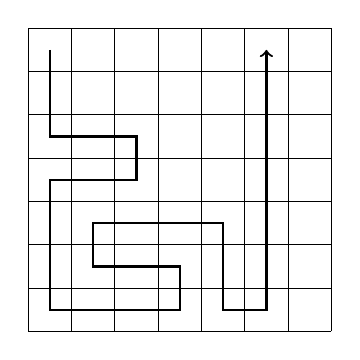
\begin{tikzpicture}[scale=.55]
  \begin{scope}
    \draw (0, 0) grid (7, 7);
    \draw[thick,->] (0.5,6.5) -- (0.5,4.5) -- (2.5,4.5) --
          (2.5,3.5) -- (0.5,3.5) -- (0.5,0.5) --
          (3.5,0.5) -- (3.5,1.5) -- (1.5,1.5) --
          (1.5,2.5) -- (4.5,2.5) -- (4.5,0.5) --
          (5.5,0.5) -- (5.5,6.5);
  \end{scope}
\end{tikzpicture}
\end{center}
Neste caso, não podemos mais visitar todos os quadrados,
então podemos encerrar a busca.
Esta otimização é muito útil:

\begin{itemize}
\item
tempo de execução: 1.8 segundos
\item
número de chamadas recursivas: 221 milhões
\end{itemize}

\subsubsection{Otimização 4}

A ideia da Otimização 3
pode ser generalizada:
se o caminho não puder continuar em frente
mas pode virar à esquerda ou à direita,
a grade se divide em duas partes
que contêm quadrados não visitados.
Por exemplo, considere o seguinte caminho:

\begin{center}
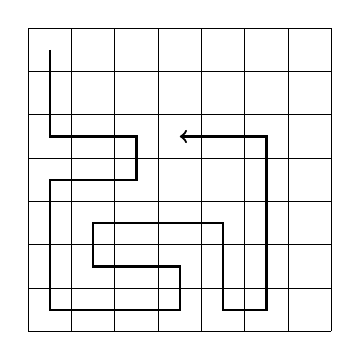
\begin{tikzpicture}[scale=.55]
  \begin{scope}
    \draw (0, 0) grid (7, 7);
    \draw[thick,->] (0.5,6.5) -- (0.5,4.5) -- (2.5,4.5) --
          (2.5,3.5) -- (0.5,3.5) -- (0.5,0.5) --
          (3.5,0.5) -- (3.5,1.5) -- (1.5,1.5) --
          (1.5,2.5) -- (4.5,2.5) -- (4.5,0.5) --
          (5.5,0.5) -- (5.5,4.5) -- (3.5,4.5);
  \end{scope}
\end{tikzpicture}
\end{center}
É claro que não podemos mais visitar todos os quadrados,
então podemos encerrar a busca.
Após esta otimização, a busca é
muito eficiente:

\begin{itemize}
\item
tempo de execução: 0.6 segundos
\item
número de chamadas recursivas: 69 milhões
\end{itemize}

~\\
Agora é um bom momento para parar de otimizar
o algoritmo e ver o que alcançamos.
O tempo de execução do algoritmo original
foi de 483 segundos,
e agora, após as otimizações,
o tempo de execução é de apenas 0.6 segundos.
Assim, o algoritmo se tornou quase 1000 vezes
mais rápido após as otimizações.

Este é um fenômeno usual em backtracking,
porque a árvore de busca é geralmente grande
e até mesmo observações simples podem efetivamente
podar a busca.
Especialmente úteis são as otimizações que
ocorrem durante as primeiras etapas do algoritmo,
ou seja, no topo da árvore de busca.

\section{Encontro no meio}

\index{encontro no meio}

\key{Encontrar no meio} é uma técnica
onde o espaço de busca é dividido em
duas partes de tamanho aproximadamente igual.
Uma busca separada é realizada
para ambas as partes,
e finalmente os resultados das buscas são combinados.

A técnica pode ser usada
se houver uma maneira eficiente de combinar os
resultados das buscas.
Nessa situação, as duas buscas podem exigir menos
tempo do que uma busca grande.
Tipicamente, podemos transformar um fator de $2^n$
em um fator de $2^{n/2}$ usando a técnica de encontro no meio.

Como exemplo, considere um problema onde
recebemos uma lista de $n$ números e
um número $x$,
e queremos descobrir se é possível
escolher alguns números da lista de modo que
sua soma seja $x$.
Por exemplo, dada a lista $[2,4,5,9]$ e $x=15$,
podemos escolher os números $[2,4,9]$ para obter $2+4+9=15$.
No entanto, se $x=10$ para a mesma lista,
não é possível formar a soma.

Um algoritmo simples para o problema é
percorrer todos os subconjuntos dos elementos e
verificar se a soma de qualquer um dos subconjuntos é $x$.
O tempo de execução de tal algoritmo é $O(2^n)$,
porque existem $2^n$ subconjuntos.
No entanto, usando a técnica de encontro no meio,
podemos alcançar um algoritmo de tempo $O(2^{n/2})$ mais eficiente\footnote{Esta
ideia foi introduzida em 1974 por E. Horowitz e S. Sahni \cite{hor74}.}.
Observe que $O(2^n)$ e $O(2^{n/2})$ são complexidades
diferentes porque $2^{n/2}$ é igual a $\sqrt{2^n}$.

A ideia é dividir a lista em
duas listas $A$ e $B$ tais que ambas
as listas contenham cerca de metade dos números.
A primeira busca gera todos os subconjuntos
de $A$ e armazena suas somas em uma lista $S_A$.
Da mesma forma, a segunda busca cria
uma lista $S_B$ a partir de $B$.
Depois disso, basta verificar se é possível
escolher um elemento de $S_A$ e outro
elemento de $S_B$ tal que sua soma seja $x$.
Isso é possível exatamente quando há uma maneira de
formar a soma $x$ usando os números da lista original.

Por exemplo, suponha que a lista seja $[2,4,5,9]$ e $x=15$.
Primeiro, dividimos a lista em $A=[2,4]$ e $B=[5,9]$.
Depois disso, criamos as listas
$S_A=[0,2,4,6]$ e $S_B=[0,5,9,14]$.
Neste caso, a soma $x=15$ é possível de formar,
porque $S_A$ contém a soma $6$,
$S_B$ contém a soma $9$, e $6+9=15$.
Isso corresponde à solução $[2,4,9]$.

Podemos implementar o algoritmo de modo que
sua complexidade de tempo seja $O(2^{n/2})$.
Primeiro, geramos listas \emph{ordenadas} $S_A$ e $S_B$,
o que pode ser feito em tempo $O(2^{n/2})$ usando uma técnica semelhante à da mesclagem.
Depois disso, como as listas estão ordenadas,
podemos verificar em tempo $O(2^{n/2})$ se
a soma $x$ pode ser criada a partir de $S_A$ e $S_B$.
